%Interaction between two individual elements in a system are %affected by the interface which is connecting the two parts.
There are different ways in which a system interact with its environment and the other systems. The interaction happening at the various boundaries are called the system's external interfaces. The boundaries between individual components inside the system are called system's internal interfaces.\\
The external and internal identification can fall into different types such as: electrical, mechanical, real-time data transfer and storage-and-retrieval of data. All the interfaces illustrated in figure. ~\ref{fig:sigFlowDiagram}.
\begin{figure}[h]
	\centering
	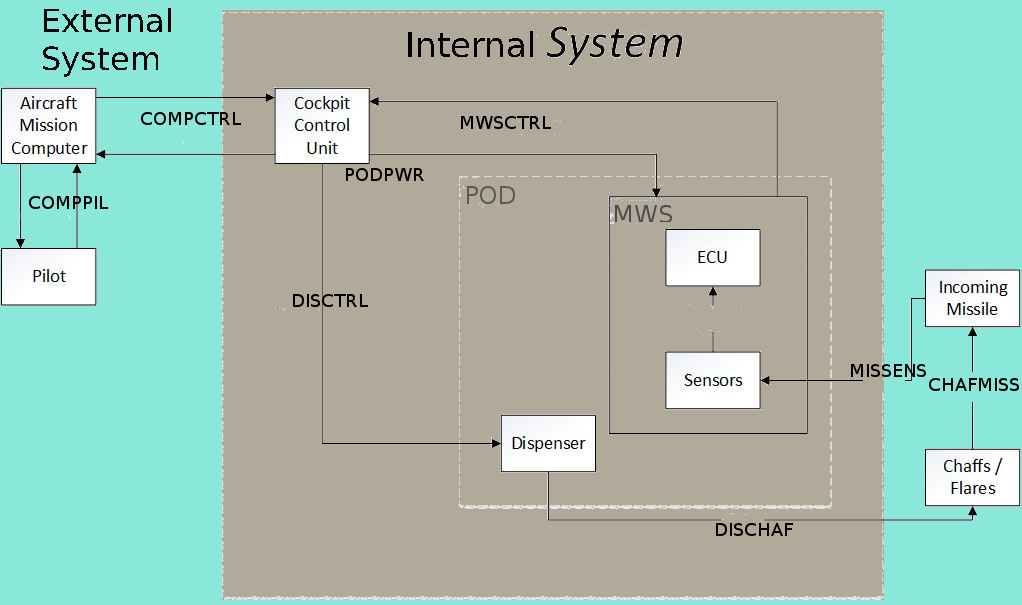
\includegraphics[scale=0.5]{./images/SignalFlowDiagramDDD_v2}\\
	\caption{Signal Flow Diagram}
    \label{fig:sigFlowDiagram}
\end{figure}

\subsubsection{External interfaces}
External interfaces are the interaction between the missile and the sensors, chaffs/flares and the dispensers, cockpit control unit and the aircraft computer, and lastly the pilot an the computer.
\begin{itemize}
\item {Interface identification and diagrams.}\\
The system interfaces listed and identified on table. ~\ref{tab:External}.


\begin{center}
\begin{table}[h]
\caption{External interface units}
\label{tab:External}
\begin{tabular}{ | p{2cm} | l | p{2.3cm} | p{2.3cm} | l | p{1cm} |}
\hline
 \textbf{Interface name} & \textbf{Identification} & \textbf{Endpoint A} & \textbf{Endpoint B} & \textbf{Standard}\\ \hline
Computer Pilot interaction & E-IF-COMPPIL & Mission computer/ Pilot & Pilot/Mission computer & \\ \hline
 Computer control & E-IF-COMPCTRL & Cockpit unit/ Mission computer &Mission computer/Cockpit unit & \\ \hline
Missile sensor input & E-IF-MISSENS & Cockpit unit & MWS & \\ \hline
Chaffs/flares missile disturbance& E-IF-CHAFMISS & Chaffs and flares & Incoming missile & \\ \hline
Dispenser Chaffs control & E-IF-DISCHAF & Dispenser & Chaffs and flares & \\ \hline
\end{tabular}
\end{table}
\end{center}

\item {Project-unique identifier of interface}\\
The unique identification listed under table.~\ref{tab:External2}. 
\begin{sidewaystable}[h]
\caption{External Interface Elements}
\label{tab:External2}
\begin{tabular}{ l l l l l l l }
\hline
%Environmental&&&&&&&&\\
&Type&Interaction medium&data element&communication methods&protocols&physical compatibility\\
\hline
Incoming missile&&&&&&\\
\hline
Chaffs and flares&&&&&&\\
\hline
Aircraft Mission Computers&&&&&&\\
\hline
System Operators&&&&&&\\
\hline
Maintenance&&&&&&\\
\hline
Support&&&&&&\\
\hline
System Housing&&&&&&\\
\hline
Shipping and handling&&&&&&\\
\hline
\end{tabular}
\end{sidewaystable}
%Electrical&Mechanical&Hydraulic
\end{itemize}


\clearpage
\subsubsection{Internal interfaces}
This section describes the internal interfaces. The system interfaces can be seen on figure \ref{fig:sigFlowDiagram}. The internal interfaces are listed in Table \ref{tab:internal}.

\begin{center}
\begin{table}[h]
\caption{Internal interfaces}
\label{tab:internal}
\begin{tabular}{ | p{2cm} | l | p{2.3cm} | p{2.3cm} | l | p{1cm} |}
\hline
 \textbf{Interface name} & \textbf{Identification} & \textbf{Endpoint A} & \textbf{Endpoint B} & \textbf{Standard}\\ \hline
 MWS Control & I-IF-MWSCTRL & Cockpit control unit & MWS & MIL-STD-1553-B\\ \hline
 Dispenser Control & I-IF-DISCTRL & Cockpit control unit & Dispenser assembly & MIL-STD-1553-B\\ \hline
 Pod power control & I-IF-PODPWR & Cockpit control unit & Dispenser assembly and MWS & N/A (electrical)\\ \hline
\end{tabular}
\end{table}
\end{center}

\paragraph{I-IF-MWSCTRL}\mbox{}\\
This real-time data transfer interface connects the cockpit control unit and missile warning system (MWS) in the pod. The interface is used to extract threat information from the MWS. The interface also provides the MWS with aircraft navigation data.
Communication on this interface is formatted as specified by MIL-STD-1553-B.
\\
The data exchanged through this interface can be seen below:
\begin{itemize}
\item Threat data (MWS $\rightarrow$ Cockpit control unit)
	\begin{itemize}
	\item Direction relative to north
	\item Size
	\item Velocity
	\end{itemize}
\item Aircraft navigation data (Cockpit control unit $\rightarrow$ MWS)
	\begin{itemize}
	\item Altitude
	\item Heading
	\item Position data
	\end{itemize}
\end{itemize}
The physical layer is defined by the MIL-STD-1553-B standard.

\paragraph{I-IF-DISCTRL}\mbox{}\\
This real-time data transfer interface connects the cockpit control unit and the dispenser assembly in the pod. The interface is used to control payload dispensing.
The data on this connection flows only from the cockpit control unit to the dispenser assembly. Communication on this interface is formatted as specified by MIL-STD-1553-B. Any data transaction on this interface is command to fire containing the following data:
\begin{itemize}
\item Direction to dispense (forwards, downwards, left, right) relative to aircraft heading. 
\item Payload selection (chaffs/flares)
\item Pattern to fire
\end{itemize}
The physical layer is defined by the MIL-STD-1553-B standard.

\paragraph{I-IF-PODPWR}\mbox{}\\
This electrical signal connects from the cockpit unit to the dispenser assembly and the MWS in the pod. When asserted, this signal enables power to the dispenser assembly and MWS. When not asserted, the power is off.